\subsection{Evaluation}\label{conflict_evaluation}
In this section, we address two research questions (RQs) and explain how we designed and conducted the experiments for each question. We then analyse the results to answer these RQs, discuss their significance and share the findings from the results.
\subsubsection*{Research Questions}
The RQs addressed in this section are as follows:
\begin{itemize}
	\item \textbf{RQ 1}: Does our tool consistently identify conflicts between USs?
	\item \textbf{RQ 2}: How does the performance of the tool change as the count of USs in a backlog increases?
	\end{itemize}
\subsubsection*{Methodology}
To answer the RQ1, "Does our tool consistently detect conflicts between USs?", we recapitulate the methodology used to analyse conflicts between USs. We used a systematic approach that includes several important steps:
\begin{itemize}
	
	\item Data Collection: For a comprehensive assessment, we applied our approach to 19 backlog datasets presented by Mosser et al. \footnote{\href{https://github.com/ace-design/nlp-stories}{https://github.com/ace-design/nlp-stories}}. They applied the Doccano approach to these publicly available requirements datasets \cite{requirementsdatasets}.
	
	 It is also worth noting that some backlog datasets (g02, g13, g17, g27) did not follow the expected sentence structure, so we did not include them in the evaluation results to avoid unexpected behaviour. Table \ref{tb:conflcit_backlogs} shows the project number of each dataset and the count of USs.
	 
	 %empty line here
	\begingroup
	\centering
	\scriptsize
	\renewcommand{\arraystretch}{1.5} 
	\begin{tabularx}{\linewidth}{l|XXXXXXXXXXXXXXXXXXX X}
		Item&	1&	2&	3&	4&	5&	6&	7&	8&	9&	10&	11&	12&	13&	14&	15&	16&	17&	18&	19&	\\
		\hline
		Project Nr.&	g03	&g04	&g05	&g08	&g10	&g11	&g12	&g14	&g16	&g18	&g19	&g21	&g22	&g23	&g24	&g25	&g26	&g27	&g28	&Total USs\\
		\hline
		Total USs&	57&	51	&53	&66	&97	&73	&54	&67	&66	&102	&137	&69	&83	&56	&53	&100	&100	&114	&60	&1458 \\
		\caption{Project number and count of USs contained in each backlog dataset}\label{tb:conflcit_backlogs}
	\end{tabularx}	
	\endgroup
	\item Splitting the elements of the US into main and benefit parts: each element of the US (action, entity and relations) was split into main or benefit part, where the main part represents the core functionality and the benefit part describes the value for the persona. In this analysis, we only consider the conflicts between the main parts of the USs.
	
	\item Recognition of conflicts: Detection of conflicts between USs in main parts of the USs based on defined criteria.
	
\end{itemize}
\subsubsection*{Ground Truth}
To answer the first research question (RQ), our automated system needs a reference point to measure its accuracy. This reference point, called "ground truth", comes from a personal judgement and serves as a benchmark for evaluating the tool's performance.

Unlike the tool evaluation, we did not assess conflicts based on defined criteria. Instead, in the ground truth evaluation, we examined conflicts based on the text of the US-pairs detected by tool. This involved reading the text of the USs and evaluating conflicts between US-pairs in a semantic manner.

The ground truth serves as the final assessment against which the automated results are compared. It results from the personal judgement of a subject matter expert (in this case me) using a combination of expertise and experience. This personal judgement is intended to provide a reliable and accurate reference for identifying conflicts between USs.\\\\
Table \ref{tb:conflict_ground_truth} shows the summary of conflicting US-pairs as ground truth.
\begin{figure}[h]
	\begingroup
	\scriptsize
	\centering
	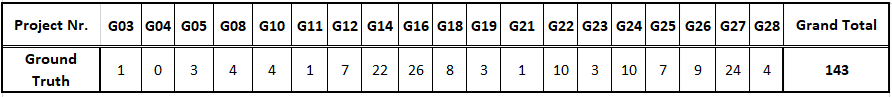
\includegraphics[scale=0.6]{Table/conflict_ground_truth.png}
	\captionof{table}{Details of the count of correctly recognised and validated conflicting US-pairs by the tool as ground truth}\label{tb:conflict_ground_truth}	
	\endgroup
\end{figure}
\subsubsection*{Evaluating Tool-Detected Conflicts Using Ground Truth}
The automated tool was developed to recognise conflicts between USs based on predefined criteria. It analyses the structure of USs to identify discrepancies that could indicate a conflict.

In contrast to ground truth, which is based on the semantic comparison of texts in the main parts of USs, the evaluation of the tool relies heavily on specified labelling (targets, triggers, contains) using the Doccano tool and predefined criteria.

Table \ref{tb:tool} shows the aggregation of the conflicting US-pairs found in the main parts evaluated by the tool.
\begin{figure}[h]
	\begingroup
	\scriptsize
	\centering
	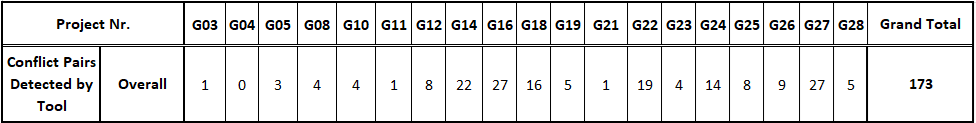
\includegraphics[scale=0.55]{Table/conflict_tool.png}
	\captionof{table}{Overall count of conflicting US-pairs in relation to the main parts assessed by the tool}\label{tb:conflict_tool}
	\endgroup
\end{figure}
\paragraph{Assessment of Result: High-Level Overview}When comparing the results provided by the tools with the ground truth, we found that 143 cases were correctly assessed as conflicting US-pairs and 30 cases were invalid on the basis of the ground truth.

Table \ref{tb:conflict_difference} shows the count of valid and invalid conflicting US-pairs assessed by the ground truth and recognised by the tool.

Based on the datasets provided, 173 conflicting US-pairs were found across all projects, with the highest count found in the backlog G27 dataset (24 cases), indicating a significant occurrence of conflicts in the USs of this project.
\begin{figure}[h]
	\begingroup
	\scriptsize
	\centering
	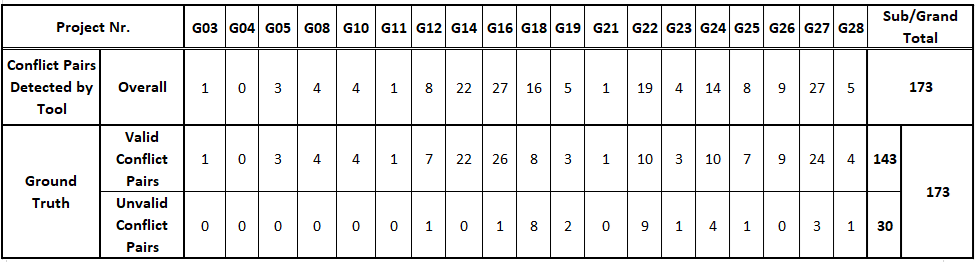
\includegraphics[scale=0.55]{Table/conflict_difference.png}
	\captionof{table}{Information on the number of discrepancies between the result provided by the tool and the ground truth}\label{tb:conflict_difference}
	
	\endgroup
\end{figure}
\paragraph{Assessment of Result: Detailed Insights}In the USs of the datasets, there are some verbs such as "have", "know" and nouns such as "data", "resource", "collection", "list", and "file" that are cross-contextual, so they do not contain generic information, which has a very negative impact on conflicts analysis (30 cases are false positives).

\begin{example}
	For example, user\_story\_983 and user\_story\_989 are reported as a conflicting US-pair in the G24 backlog dataset:\\
	\textit{user\_story\_1365:} \#G24\# As a depositor, I want to store and manage \#datasets\# via a simple web interface.\\
	\textit{user\_story\_1409:} \#G24\# As a research information manager, I want to have \#datasets\# linked to metadata about projects.\\
	The depositor needs a simple interface for uploading and managing datasets. The research information manager needs to be able to link these datasets to comprehensive metadata about the projects.\\
	These needs are not inherently conflicting, but they require careful design consideration to ensure that both needs are met effectively.\\
	To avoid the conflict, the verb "have" related to "user\_story\_1409" should be defined more precisely. The US should be amended as follows:\\
	\textit{user\_story\_1409:} \#G24\# As research information manager, I want to \textit{\texttt{link} \texttt{datasets}} to metadata about projects.\\
\end{example}

There are also annotated USs with inaccurate labelling by the Doccano tool. In other words, there is more information about the resource in concern provided in US, which leads to inconsistencies and bias.
\begin{example}
	In the dadaset of backlog G25, for example, we have a US-pair that are marked as conflict:\\
	\textit{user\_story\_1506}: \enquote{\#G25\# As a DAMS manager, I want to know when the \#application\# of a statute to an object or object component has been \#modified\#, either manually or automatically.}\\
	\textit{user\_story\_1510:} \enquote{\#G25\# As a DAMS manager, I want to know if \#application\# of a library policy to an object or object component has been \#modified\#, either manually or automatically.}\\
	In the annotated dataset, the identified entities of "user\_story\_1506" and "user\_story\_1510" are only \enquote{application}, which is not fully labelled. The correct labelling for "user\_story\_1506" should be \texttt{"application of a statute"} and for "user\_story\_1510" should be \texttt{"application of a library policy"}. With these changes, no conflict will be reported between these two USs.
\end{example}
\paragraph{RQ1: Conclusion}
After comparing the ground truth result with the result provided by our tool, we find that 83\% of the conflicting US-pairs found are valid and only 17\% of the cases are invalid which is classically considered as excellent.

The results of the automated tool are consistent with the ground truth, which shows that it reliably recognises conflicts. This agreement with personal judgements increases confidence in the accuracy and validity of the tool. 

The tool also demonstrates its effectiveness and trustworthiness. This reliability means that users can rely on the tool to accurately identify conflicts, reducing the need for extensive manual review. 
\subsubsection*{Performance Evaluation}
To answer the RQ2 "How does the performance of the tool change as the count of USs in a backlog increases?", we conducted a series of tests to measure the time it takes the tool to process different counts of USs. This section describes the test method, the results obtained and the impact on the scalability of the tool.
\paragraph{Test Methodology}To evaluate the tool's performance, we conducted a set of experiments in which the tool processed different numbers of USs in a backlog. The tests involved the following steps:
\begin{enumerate}
	\item Backlog Setup: We used backlogs with varying numbers of USs around—50, 70, 90, 120 and 140—to simulate different workload sizes. Each backlog contained USs with varying content, and complexity to represent a realistic range of cases. Table \ref{tb:conflict_performance_env} shows information on the backlog data records provided for the performance test application.
	\begin{figure}[h]
		\begingroup
		\scriptsize
		\centering
		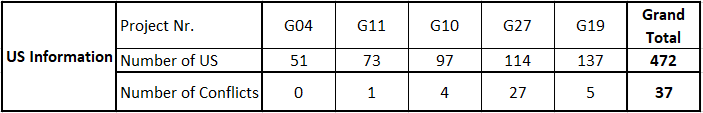
\includegraphics[scale=0.7]{Table/conflict_performance_env.png}
		\captionof{table}{Information on the backlog datasets provided for the application of the performance test}\label{tb:conflict_performance_env}
		\endgroup
	\end{figure}
	\item Tool Execution: Each part of toolchain (USPartExtractor, ActionsAnnotationsCreator, and ReportMaker) was run for each backlog and the total time taken to process the entire backlog was recorded. The performance of the tool was measured by the processing time, i.e. the total time taken to process all USs in the backlog and identify conflicts and reporting.
	
	\item Repeating Tests: To ensure reliability, each test was conducted multiple times, and the average processing time was calculated.
\end{enumerate}
The test environment consisted of:
\begin{itemize}
	\item Processor: Intel(R) Core(TM) i7-8565U CPU @ 1.80GHz (8 CPUs), ~2.0GHz		
	\item Memory: 8070MB RAM
	\item Display Devices: Intel(R) UHD Graphics 620, 4163 MB(Display Memory)
	\item Hard Disk: INTEL SSDPEKNW512G8H
	\item Operating System: Windows 11 Home 64-bit (10.0, Build 22631) (22621.ni\_release .220506-1250)
	\item System Type: 64-bit operating system, x64-based processor
\end{itemize}
Table \ref{tb:conflict_performance_result} shows the result of tool's performance in seconds which were conducted on a controlled environment to ensure consistency.
	\begin{figure}[h]
	\begingroup
	\scriptsize
	\centering
	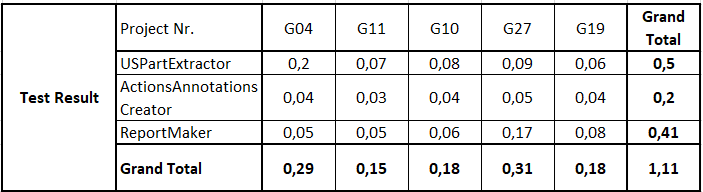
\includegraphics[scale=0.75]{Table/conflict_performance_result.png}
	\captionof{table}{Information about the result of the tool's performance test, which was measured using the processing time in seconds.}\label{tb:conflict_performance_result}
	\endgroup
\end{figure}
\paragraph{RQ2: Conclusion}There is no direct relationship between the count of USs in a backlog and the processing time required by our tool (G27 vs G19).
However, there is a direct relationship between the count of conflicts found between USs and the processing time. The more conflicts there are, the longer the processing time. 

Overall, developers and project managers with a growing backlog can expect the tool to take a reasonable amount of time to assess conflicts.
\subsubsection*{Threats to Validity}
Several potential threats to validity need to be considered when assessing the conflicts between USs both by personal judgement (ground truth) and by the automated tool. This section outlines the main threats to validity and describes how they were mitigated during the study.
\paragraph{Construct validity}It refers to how accurately the assessment measures what it is supposed to measure. The following risks have been identified:
\begin{itemize}
	\item Ambiguity of criteria: If the criteria for conflict are unclear or open to interpretation, this can lead to inconsistent scores. To avoid this, we defined clear and detailed criteria for identifying conflicts in USs.
	
	\item Ambiguity of action-annotations: If the action-annotations associated with each verb in a US are unclear or not specific to the context, this can lead to inconsistent scores. To prevent this, we assign the action-annotations based on the context of the backlog instead of using general terms.
	
	\item Subjectivity in ground truth: Since the ground truth is based on personal judgements, subjectivity could lead to bias. To minimise this risk, the evaluator (in this case me) has cross-checked the evaluations several times.
\end{itemize}
\paragraph{External validity}External validity refers to how well the results of the study can be transferred to other contexts or populations. Threats to external validity include:

\begin{itemize}
	\item specificity of USs: If the USs in the study are too specific or specific to the context, the results may not be transferable to other projects. To avoid this, we analysed 19 backlog datasets with different USs and project types.
	
	\item Tool Limitations:
	\begin{itemize}
		
	 \item The automated tool is tailored to a specific format of USs, which limits its wider applicability. It is highly dependent on the exact structure of USs (e.g. "As \textless role\textgreater I want to ..., so that ..."), which is crucial for its functionality. Therefore, we evaluated the tool in controlled environments, focussing exclusively on well-structured USs, and investigated its performance in different scenarios.
	
	\item Our tool relies on a specific type of annotations for USs, e.g. action, entity, their reference targets, triggers and contains. The effectiveness of the tool depends on these annotations being accurate and consistent. If the annotations are incomplete or incorrect, the tool may not work properly. Also, the tool may not be compatible with other annotation schemes that use different labels.
	
	\item The verbs in the action-annotation reference database are not included in their root form, but as they actually occur in the USs. This means that the same verb in different forms may be found in the database.
\end{itemize}
\end{itemize}
\paragraph{Internal Validity}Internal validity is concerned with whether the observed results are attributable to the factors analysed or are influenced by other variables. Potential threats to internal validity include:
\begin{itemize}
	\item Confounding factors: External factors or unintended variables can influence the evaluation of the conflicts analysis. In particular, the USs annotated with Doccano have a significant influence on the conflicts analysis. The more phrases are covered as label (especially as entity and action), the better the result of evaluation. Since our tool uses Doccano-annotated USs without changes as primary input, these discrepancies are unavoidable.
	
	\item Limitation of tool: The automated tool does not take into account the analysis of conflicts in the benefit parts of the USs.
\end{itemize}
\subsection{Conclusion}\label{conflict_conclustion}
In this study, we introduced an approach that integrates the Doccano tool and our custom tool to systematically identify and report conflicts between USs in software development projects. We also conducted an evaluation of this approach.

By carefully analysing 19 different backlog datasets, our method not only separated the USs into main and benefit parts for nuanced examination, but also facilitated conflicts analysis by translating the verbs of the main parts into four distinct categories, namely "delete", "create", "forbid" and "preserve", and finally reported the potential conflicts in text base format.

Our results reveal a decisive finding: the effectiveness of conflicts analysis is significantly influenced by the quality of the USs and their annotations. Well-formulated USs, in which general verbs (e.g. "have", "know") and nouns (e.g. "data", "list", "collection") are avoided, as well as a concisely annotated backlog with precise labelling of the entities (nouns) significantly improve the effectiveness of the conflicts analysis.

 If the main parts of a US-pair contradict each other, the application of one US has a negative effect on another US by deleting a resource that another US uses, or creating a resource that another US prohibits, or deleting a resource that another US also wants to delete.
 
 If conflicts between USs are identified, this is a signal for the project team to take a closer look at the requirements and the design of the system. By prioritising, sequencing, defining clear rules, implementing conflict resolution mechanisms, refining USs and involving stakeholders, the team can effectively manage and resolve these conflicts to ensure a well-functioning system.
 
In summary, our study confirms the central role of a semantic analysis approach in the detection and management of conflicts in project backlogs and thus contributes to the rationalisation of software development processes.

The quality of the annotated USs and their well-formed structure are central to the success of this approach. The results of this study provide useful guidance for improving current practices and shaping future research in software project management.
